\renewcommand{\thefootnote}{\fnsymbol{footnote}}

\chapter[First theorem of welfare economics]%
 {First theorem of welfare economics}%
\label{ch:L8}

% 3) Reset things so later footnotes go back to 1, 2, 3, …
%\setcounter{footnote}{0}
\renewcommand{\thefootnote}{\arabic{footnote}}

%\section{A preliminary lemma}\label{sec:L8-intro}

In this lecture we discuss the first theorem of welfare economics, which states that every Walrasian equilibrium with transfers is \usename{axn:po}. We now start seeing proofs that are a bit more sophisticated.\footnote{An immensely valuable resource to learn fundamental proof strategies is \cite{cummingsProofsLongFormMathematics2021}. If you want to have fun and understand Italian, you can read \cite{lolliQEDFenomenologiaDimostrazione2020}.} In particular, we will make use of proofs \textit{by contradiction}. The logic is as follows. We want to prove a statement \( S \). We assume that \( S \) is false and show that this assumption leads to a contradiction: for instance, we derive a conclusion of the form \( C \) and \textbf{not} \( C \), or we obtain a conclusion that contradicts one of the premises needed for \( S \). Either way, the assumption that \( S \) is false cannot be sustained, so \( S \) must be true.

We begin with a preliminary lemma.

\begin{lemma}\label{lem:lns}
    Assume that preferences \( \succsim_i \) are locally non-satiated. Let \( x_i \in D_i(p,e_i) \). If \( x'_i \succsim_i x_i \), then \( p \cdot x'_i \ge p \cdot x_i \).
\end{lemma}

\begin{proof}
    Suppose, to the contrary, that \( p \cdot x'_i < p \cdot x_i \). Let

    \[
        \delta = \frac{p \cdot x_i - p \cdot x'_i}{2} > 0.
    \]

    By \usename{axn:lns}, for every \( \varepsilon > 0 \) there exists \( x''_i \in \mathbb{R}^{\ell}_{+} \) such that \( \|x''_i - x'_i\| < \varepsilon \) and \( x''_i \succ_i x'_i \).

    Choose \( \varepsilon \) small enough so that \( \|x''_i - x'_i\| < \varepsilon \) implies \( |p \cdot x''_i - p \cdot x'_i| < \delta \). Then

    \[
        p \cdot x''_i \le p \cdot x'_i + \delta < p \cdot x_i .
    \]

    Since \( x_i \in D_i(p,e_i) \), we have \( p \cdot x_i \le p \cdot e_i \), hence \( p \cdot x''_i < p \cdot e_i \) and therefore \( x''_i \in B(p,e_i) \).
    Moreover, \( x''_i \succ_i x'_i \) and \( x'_i \succsim_i x_i \) imply \( x''_i \succ_i x_i \) by transitivity. This contradicts the fact that \( x_i \in D_i(p,e_i) \).
\end{proof}

And now the main result.

\begin{theorem}\label{thm:fftwe} (\textbf{First theorem of welfare economics})
    If preferences in economy \( E \) are locally non-satiated, then every allocation selected by \( R^{WT} \) is \usename{axn:po}. That is,
    \[
        x \in R^{WT}(E) \quad \Longrightarrow \quad x \text{ is \usename{axn:po}}.
    \]
\end{theorem}

\begin{proof}
    Let \(E\) be an economy and suppose that \(x \in R^{WT}(E)\). Then there exist strictly positive prices \(p\) and transfers \((T_i)_{i}\) such that, for every individual \(i\),

    \[
        x_i \in D_i(p, e_i + T_i),
    \]

    that is, \(x_i\) is a most preferred bundle in the budget set \(B(p, e_i + T_i)\).

    Suppose, for a contradiction, that \(x\) is not \usename{axn:po}. Then there exists a feasible allocation \(x'\) such that \(x'_i \succsim_i x_i\) for all \(i\), and \(x'_j \succ_j x_j\) for some individual \(j\). By Lemma~\ref{lem:lns}, this implies

    \[
        p\cdot x'_i \ge p\cdot x_i \quad \text{for all } i.
    \]

    Moreover, for the individual \(j\) with \(x'_j \succ_j x_j\) we in fact have \(p\cdot x'_j > p\cdot x_j\): if \(p\cdot x'_j \le p\cdot x_j\), then \(x'_j \in B(p,e_j+T_j)\), since \(x_j \in B(p,e_j+T_j)\), contradicting \(x_j \in D_j(p,e_j+T_j)\). Therefore,

    \[
        p\cdot x'_j > p\cdot x_j \quad \text{for some } j.
    \]

    Summing over all individuals,

    \begin{equation}
        \sum_{i} p\cdot x'_i > \sum_{i} p\cdot x_i .
        \tag{*}
    \end{equation}

    On the other hand, local non-satiation implies that each demanded bundle exhausts the budget, so \(p\cdot x_i = p\cdot(e_i+T_i)\) for all \(i\). Summing and using \(\sum_i T_i = 0\),

    \[
        \sum_i p\cdot x_i \;=\; \sum_i p\cdot(e_i+T_i) \;=\; \sum_i p\cdot e_i .
    \]

    Since \(x'\) is feasible, \(\sum_i x'_i \le \sum_i e_i\), and multiplying by the strictly positive price vector \(p\) gives

    \[
        \sum_i p\cdot x'_i \;\le\; \sum_i p\cdot e_i \;=\; \sum_i p\cdot x_i,
    \]

    contradicting \((*)\). Hence no such \(x'\) exists, and \(x\) is \usename{axn:po}.
\end{proof}

Before turning to the interpretation of Theorem~\ref{thm:fftwe}, let us discuss why \usename{axn:lns} is necessary for the theorem to hold. Look at Figure~\ref{fig:lns-welf}. Individual \(1\) has \textquote{thick} indifference curves, so he violates local non-satiation. The allocation \(x\) is not \usename{axn:po}, since there is another feasible allocation \(x'\) that makes individual \(2\) strictly better off without making individual \(1\) worse off. However, \(x\) can still be supported as a \usename{axn:weqt} at prices \(p\). Thus, without local non-satiation, Theorem~\ref{thm:fftwe} fails.

\begin{figure}[H]
    \begin{center}
        \tikzset{every picture/.style={line width=0.75pt}} %set default line width to 0.75pt        

        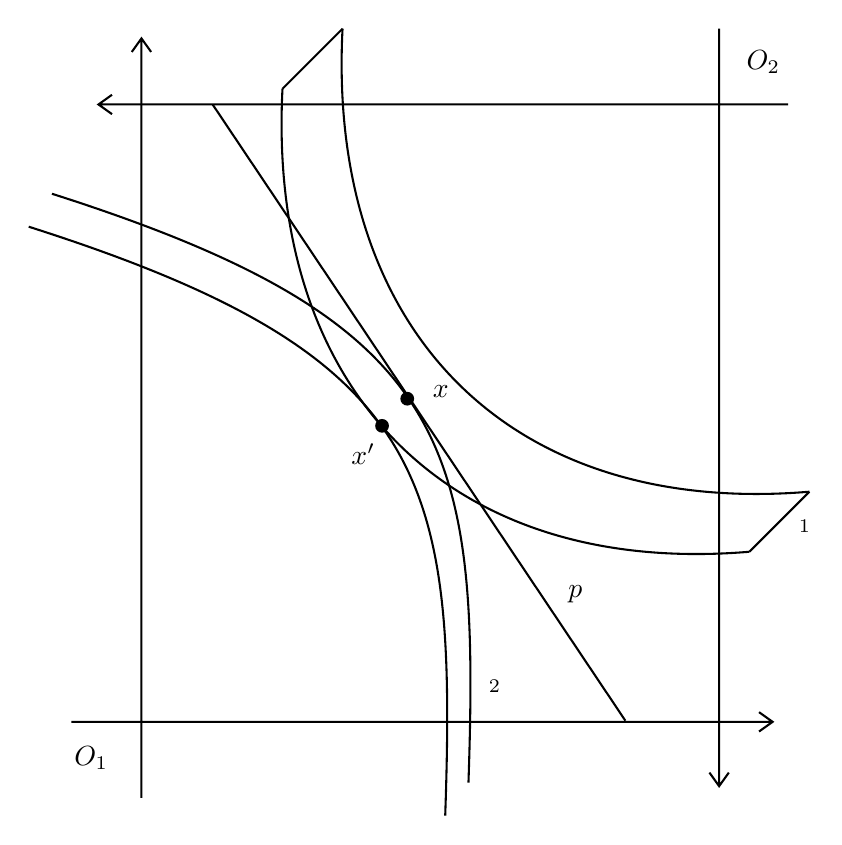
\begin{tikzpicture}[x=0.70pt,y=0.70pt,yscale=-1,xscale=1]
            %uncomment if require: \path (0,443); %set diagram left start at 0, and has height of 443

            %Shape: Axis 2D [id:dp22115699468612893] 
            \draw  (140,370.4) -- (502,370.4)(176.2,17.6) -- (176.2,409.6) (495,365.4) -- (502,370.4) -- (495,375.4) (171.2,24.6) -- (176.2,17.6) -- (181.2,24.6)  ;
            %Shape: Axis 2D [id:dp32207533916759135] 
            \draw  (510,51.7) -- (154,51.7)(474.4,403.6) -- (474.4,12.6) (161,56.7) -- (154,51.7) -- (161,46.7) (479.4,396.6) -- (474.4,403.6) -- (469.4,396.6)  ;
            %Curve Lines [id:da8559403196511832] 
            \draw    (249,43.6) .. controls (241,199.6) and (335,295.6) .. (490,282.6) ;
            %Curve Lines [id:da37662840950707166] 
            \draw    (280,12.6) .. controls (272,168.6) and (366,264.6) .. (521,251.6) ;
            %Straight Lines [id:da5642668535456735] 
            \draw    (249,43.6) -- (280,12.6) ;
            %Straight Lines [id:da9097139754709688] 
            \draw    (490,282.6) -- (521,251.6) ;
            %Curve Lines [id:da09819389723996741] 
            \draw    (130,97.8) .. controls (337,163.8) and (351,225.8) .. (345,401.8) ;
            %Shape: Circle [id:dp16582666368555876] 
            \draw  [fill={rgb, 255:red, 0; green, 0; blue, 0 }  ,fill opacity=1 ] (310.4,203.6) .. controls (310.4,201.94) and (311.74,200.6) .. (313.4,200.6) .. controls (315.06,200.6) and (316.4,201.94) .. (316.4,203.6) .. controls (316.4,205.26) and (315.06,206.6) .. (313.4,206.6) .. controls (311.74,206.6) and (310.4,205.26) .. (310.4,203.6) -- cycle ;
            %Shape: Circle [id:dp20605667579120546] 
            \draw  [fill={rgb, 255:red, 0; green, 0; blue, 0 }  ,fill opacity=1 ] (297.4,217.6) .. controls (297.4,215.94) and (298.74,214.6) .. (300.4,214.6) .. controls (302.06,214.6) and (303.4,215.94) .. (303.4,217.6) .. controls (303.4,219.26) and (302.06,220.6) .. (300.4,220.6) .. controls (298.74,220.6) and (297.4,219.26) .. (297.4,217.6) -- cycle ;
            %Curve Lines [id:da6954752398238686] 
            \draw    (118,114.8) .. controls (325,180.8) and (339,242.8) .. (333,418.8) ;
            %Straight Lines [id:da49767621503014337] 
            \draw    (213,51.8) -- (426,369.8) ;

            % Text Node
            \draw (140,381.4) node [anchor=north west][inner sep=0.75pt]    {$O_{1}$};
            % Text Node
            \draw (487,22.4) node [anchor=north west][inner sep=0.75pt]    {$O_{2}$};
            % Text Node
            \draw (514,264.4) node [anchor=north west][inner sep=0.75pt]    {$\succsim _{1}$};
            % Text Node
            \draw (325,195.4) node [anchor=north west][inner sep=0.75pt]    {$x$};
            % Text Node
            \draw (283,225.4) node [anchor=north west][inner sep=0.75pt]    {$x'$};
            % Text Node
            \draw (354,347.4) node [anchor=north west][inner sep=0.75pt]    {$\succsim _{2}$};
            % Text Node
            \draw (395,298.4) node [anchor=north west][inner sep=0.75pt]    {$p$};
        \end{tikzpicture}
        \caption{Local non-satiation is necessary for the First Welfare Theorem.}
        \label{fig:lns-welf}
    \end{center}
\end{figure}

\begin{techremark}
    Why can \(x\) be supported as a \usename{axn:weqt} in Figure~\ref{fig:lns-welf}?
\end{techremark}

Let us now interpret Theorem~\ref{thm:fftwe}. A classical economic question is how to allocate resources given information about preferences.\footnote{In its most general form, a question of this kind is asked in \cite{arrowSocialChoiceIndividual2012}, the spark that gave rise to modern social choice theory.} We might want such an allocation of resources to satisfy some attractive properties from a \textit{normative} perspective. One such property is Pareto optimality. An allocation rule that takes preferences and endowments as inputs and returns a \usename{axn:po} allocation as output might therefore be desirable. However, once one has an allocation rule, one might wonder whether it can be implemented in a decentralised way. A rule that maps preferences and endowments into an allocation does not, by itself, tell us \textit{how} to reach that allocation.

Theorem~\ref{thm:fftwe} tells us that Walrasian equilibrium with transfers implements an allocation rule that always delivers \usename{axn:po} allocations. Decentralised individual optimisation at some prices can therefore lead to desirable allocations from this point of view. There is a bit more, however. A Walrasian equilibrium with transfers is not just a mechanism to implement \usename{axn:po} allocations. It also induces a price for each good, which individuals can use to trade in order to reach those allocations. Prices may be interpreted as \textquote{values} for goods, where these values depend on the preferences and endowments of all individuals in the economy. In fact, \cite{debreuTheoryValueAxiomatic1959} is titled \textit{Theory of Value}.

Many more or less sophisticated critiques of economics stem from the idea that it is inappropriate to view the value of goods as determined by prices. There is a famous quotation, often misattributed to Oscar Wilde,\footnote{Apparently the original quotation is \textquote{[A cynic is] a man who knows the price of everything, and the value of nothing} from \citet[p. 55]{wildeLadyWindermeresFan1995}.} that says: \textquote{An economist is someone who knows the price of everything and the value of nothing}. Of course, there are legitimate reasons to question whether values should be entirely derived from individual preferences. But, in the setting we consider here, there is nothing special about prices that is not ultimately related to preferences or endowments.\footnote{However, sometimes the mere existence of prices, from a physical point of view, induces disgust towards the commodification of goods that \textquote{should not be priced}. As \citet[p. 201]{sophoclesAntigoneSophoclesEnglish1939} puts it: \textquote{There’s nothing in the world so demoralizing as money}. \cite{fleurbaeyEfficiencyEquitySociallyembedded2025} studies a class of problems, of which commodification is one, in a general equilibrium setting, so you are ready to read it!}

Unfortunately, an allocation rule that delivers \usename{axn:po} allocations can sometimes be undesirable from other points of view. For instance, it might deliver very unequal allocations. We might therefore want to complement Pareto optimality with a distributional requirement. One candidate is envy-freeness, which is closely related to the idea of equality of opportunity. One way to make this relationship precise is captured in the following proposition.

\begin{proposition}\label{prop:envy}
    Every allocation selected by \(R^{EW}\) satisfies \usename{axn:no-envy}. That is,

    \[
        x \in R^{EW}(E) \quad \Longrightarrow \quad x \ \text{satisfies \usename{axn:no-envy}}.
    \]
\end{proposition}

\begin{proof}
    Let \(E\) be an economy and suppose that \(x \in R^{EW}(E)\). By definition of \usename{axn:weqe}, there exists a price vector \(p \in \mathbb{R}^\ell_{++}\) such that, for each individual \(i\),

    \[
        x_i \in D_i\!\left(p,\frac{\bar e}{n}\right).
    \]

    Because all individuals face the same endowment \(\frac{\bar e}{n}\) and the same price vector \(p\), they all face the same budget set

    \[
        B := B\!\left(p, \frac{\bar e}{n}\right)
        = \left\{\, x_i' \in \mathbb{R}^\ell_+ \ \middle|\ p \cdot x_i' \le p \cdot \tfrac{\bar e}{n} \,\right\}.
    \]

    Fix any individual \(i\). Since \(x_i \in D_i\!\left(p,\frac{\bar e}{n}\right)\), \(x_i\) is a most preferred bundle for \(i\) in \(B\). Therefore,

    \begin{equation}
        \label{eq:maximal}
        \text{for all } x_i' \in B,\qquad x_i \succsim_i x_i'.
    \end{equation}

    Now consider any other individual \(j\neq i\). Since \(x_j \in D_j\!\left(p,\frac{\bar e}{n}\right)\), we have \(x_j \in B\). Applying \eqref{eq:maximal} to the specific bundle \(x_j\) yields

    \[
        x_i \succsim_i x_j.
    \]

    Since \(i\) and \(j\neq i\) were arbitrary, it follows that for all \(i\neq j\),

    \[
        x_i \succsim_i x_j,
    \]

    which is exactly \usename{axn:no-envy}. Hence the allocation \(x\) satisfies \usename{axn:no-envy}.
\end{proof}

Since any \usename{axn:weqe} is also a \usename{axn:weqt}, take transfers \(T_i := \tfrac{\bar e}{n} - e_i\), Theorem~\ref{thm:fftwe} and Proposition~\ref{prop:envy} together imply that the Egalitarian Walrasian allocation rule delivers allocations that are both \usename{axn:po} and satisfy \usename{axn:no-envy}. Therefore, in this simple setting, requirements of \textit{efficiency}, \textit{fairness}, and \textit{incentives} are not incompatible!\footnote{\citet[p. 405]{thomsonFairAllocationRules2011} discusses that the Egalitarian Walrasian allocation rule is also easy to implement under incomplete information about preferences.}

However, the actual endowments \(e_i\) need not coincide with the egalitarian endowment \(\tfrac{\bar e}{n}\). We might therefore be interested in understanding when such an allocation rule can be implemented starting from an arbitrary endowment profile. The second fundamental theorem of welfare economics, which we discuss in the next lecture, provides conditions under which this is possible.

\paragraph{Things to read.} The proof of Theorem~\ref{thm:fftwe} in these notes follows \citet[pp. 545--550]{mas-colellMicroeconomicTheory1995}. A proof of a closely related version of Proposition~\ref{prop:envy} appears in \citet[p. 46]{fleurbaeyFairnessResponsibilityWelfare2008}, which also discusses further properties of allocations satisfying \usename{axn:no-envy}.

\section{Exercises}

\begin{exercise}
    Explain why Proposition~\ref{prop:envy} links envy-freeness to equality of opportunity. There are at least a couple of things to say here. For instance, do the allocations selected by the Egalitarian Walrasian allocation rule depend on individuals' endowments?
\end{exercise}

\bibliographystyle{apacite}  % or another  style
\bibliography{references} % .bib file goes in ./bib/